%%%%%%%%%%%%%%%%%%%%%%%%%%%%%%%%%%%%%%%%%
% Masters/Doctoral Thesis 
% LaTeX Template
% Version 2.5 (27/8/17)
%
% This template was downloaded from:
% http://www.LaTeXTemplates.com
%
% Version 2.x major modifications by:
% Vel (vel@latextemplates.com)
%
% This template is based on a template by:
% Steve Gunn (http://users.ecs.soton.ac.uk/srg/softwaretools/document/templates/)
% Sunil Patel (http://www.sunilpatel.co.uk/thesis-template/)
%
% Template license:
% CC BY-NC-SA 3.0 (http://creativecommons.org/licenses/by-nc-sa/3.0/)
%
%%%%%%%%%%%%%%%%%%%%%%%%%%%%%%%%%%%%%%%%%

%----------------------------------------------------------------------------------------
%	PACKAGES AND OTHER DOCUMENT CONFIGURATIONS
%----------------------------------------------------------------------------------------

\documentclass[
11pt, % The default document font size, options: 10pt, 11pt, 12pt
openany,
%oneside, % Two side (alternating margins) for binding by default, uncomment to switch to one side
english, % ngerman for German
singlespacing, % Single line spacing, alternatives: onehalfspacing or doublespacing
%draft, % Uncomment to enable draft mode (no pictures, no links, overfull hboxes indicated)
%nolistspacing, % If the document is onehalfspacing or doublespacing, uncomment this to set spacing in lists to single
%liststotoc, % Uncomment to add the list of figures/tables/etc to the table of contents
%toctotoc, % Uncomment to add the main table of contents to the table of contents
%parskip, % Uncomment to add space between paragraphs
%nohyperref, % Uncomment to not load the hyperref package
headsepline, % Uncomment to get a line under the header
%chapterinoneline, % Uncomment to place the chapter title next to the number on one line
%consistentlayout, % Uncomment to change the layout of the declaration, abstract and acknowledgements pages to match the default layout
]{Thesis} % The class file specifying the document structure

\usepackage[utf8]{inputenc} % Required for inputting international characters
\usepackage[T1]{fontenc} % Output font encoding for international characters

\usepackage{mathpazo} % Use the Palatino font by default

\usepackage[backend=bibtex,style=authoryear,natbib=true]{biblatex} % Use the bibtex backend with the authoryear citation style (which resembles APA)

\addbibresource{bibliography.bib} % The filename of the bibliography

\usepackage[autostyle=true]{csquotes} % Required to generate language-dependent quotes in the bibliography

%----------------------------------------------------------------------------------------
%	MARGIN SETTINGS
%----------------------------------------------------------------------------------------

\geometry{
	paper=a4paper, % Change to letterpaper for US letter
	inner=2.5cm, % Inner margin
	outer=3.8cm, % Outer margin
	bindingoffset=.5cm, % Binding offset
	top=1.5cm, % Top margin
	bottom=1.5cm, % Bottom margin
	%showframe, % Uncomment to show how the type block is set on the page
}

%----------------------------------------------------------------------------------------
%	THESIS INFORMATION
%----------------------------------------------------------------------------------------

\thesistitle{To What Extent Do MFCCs Perform Better Than Other Speech Feature Extraction Algorithms in Speech Recognition CNNs} % Your thesis title, this is used in the title and abstract, print it elsewhere with \ttitle
\supervisor{Courtney \textsc{Edwards}} % Your supervisor's name, this is used in the title page, print it elsewhere with \supname
\degree{International Baccalaureate Programme} % Your degree name, this is used in the title page and abstract, print it elsewhere with \degreename
\author{Daniel \textsc{Lu}} % Your name, this is used in the title page and abstract, print it elsewhere with \authorname

\subject{Computer Sciences} % Your subject area, this is not currently used anywhere in the template, print it elsewhere with \subjectname
\university{\href{https://merivalehs.ocdsb.ca/}{Merivale High School}} % Your university's name and URL, this is used in the title page and abstract, print it elsewhere with \univname

\AtBeginDocument{
\hypersetup{pdftitle=\ttitle} % Set the PDF's title to your title
\hypersetup{pdfauthor=\authorname} % Set the PDF's author to your name
}

\begin{document}

\frontmatter % Use roman page numbering style (i, ii, iii, iv...) for the pre-content pages

\pagestyle{plain} % Default to the plain heading style until the thesis style is called for the body content

%----------------------------------------------------------------------------------------
%	TITLE PAGE
%----------------------------------------------------------------------------------------

\begin{titlepage}
\begin{center}

\vspace*{.06\textheight}
{\scshape\LARGE \univname\par}\vspace{1.5cm} % University name

\HRule \\[0.4cm] % Horizontal line
{\huge \bfseries \ttitle\par}\vspace{0.4cm} % Thesis title
\HRule \\[1.5cm] % Horizontal line
 
\begin{minipage}[t]{0.4\textwidth}
\begin{flushleft} \large
\emph{Author:}\\
{\authorname} % Author name - remove the \href bracket to remove the link
\end{flushleft}
\end{minipage}
\begin{minipage}[t]{0.4\textwidth}
\begin{flushright} \large
\emph{Supervisor:} \\
{\large \supname} % Supervisor name - remove the \href bracket to remove the link  
\end{flushright}
\end{minipage}\\[3cm]
 
\vfill

{\large \today}\\[4cm] % Date

\vfill
\end{center}
\end{titlepage}

%----------------------------------------------------------------------------------------
%	LIST OF CONTENTS/FIGURES/TABLES PAGES
%----------------------------------------------------------------------------------------

\tableofcontents % Prints the main table of contents

%----------------------------------------------------------------------------------------
%	ABBREVIATIONS
%----------------------------------------------------------------------------------------

\begin{abbreviations}{ll} % Include a list of abbreviations (a table of two columns)

\textbf{LAH} & \textbf{L}ist \textbf{A}bbreviations \textbf{H}ere\\
\textbf{WSF} & \textbf{W}hat (it) \textbf{S}tands \textbf{F}or\\

\end{abbreviations}

%----------------------------------------------------------------------------------------
%	SYMBOLS
%----------------------------------------------------------------------------------------

\begin{symbols}{lll} % Include a list of Symbols (a three column table)

$a$ & distance & \si{\meter} \\
$P$ & power & \si{\watt} (\si{\joule\per\second}) \\
%Symbol & Name & Unit \\

\addlinespace % Gap to separate the Roman symbols from the Greek

$\omega$ & angular frequency & \si{\radian} \\

\end{symbols}

%----------------------------------------------------------------------------------------
%	THESIS CONTENT - CHAPTERS
%----------------------------------------------------------------------------------------

\mainmatter % Begin numeric (1,2,3...) page numbering

\pagestyle{thesis} % Return the page headers back to the "thesis" style

% Include the chapters of the thesis as separate files from the Chapters folder
% Uncomment the lines as you write the chapters

% Chapter Template

\chapter{Introduction} % Main chapter title

\label{Introduction} % Change X to a consecutive number; for referencing this chapter elsewhere, use \ref{ChapterX}

%----------------------------------------------------------------------------------------
%	ABSTRACT
%----------------------------------------------------------------------------------------

\section{Abstract}

Automatic speech recognition (ASR) is the ability of a machine to recognize language from human speech and convert it into written text. Such a task is difficult due to the sheer complexity of any spoken language, as well as the varying and unpredictable nature of different people and their speaking habits. Even big-name companies such as Alphabet, Microsoft, and Baidu, who pride themselves in their sophisticated multi-million dollar speech recognition systems, have been countlessly ridiculed for their misinterpretations. However, due to the endless number of possible and practical applications of ASR technology in our developing world, major corporations still aspire to develop an accurate yet optimized speech recognition system for their products and services. For instance, Baidu spent a total of \$4.7 billion dollars on research and development, of which a large portion headed into developing their voice assistant, DuerOS. Hence, the implementation of ASR can improve the ergonomics of any task that requires human interaction, such as personal assistants, smart healthcare and household appliances, and media transcription to support people with disabilities or language barriers. 
\newline\par
Significant development for ASR began in the 50s, with the innovation of Bell’s Audrey and IBM’s Shoebox. These systems fell into a category of ASR systems that recognized individual words to an isolated vocabulary using manually set parameters for phoneme recognition. By the end of the decade, ASR technology could distinguish words with a maximum of four vowels and nine consonants and by the 80s, systems could recognize up to 3000 words, which is around the vocabulary of a six-year-old child. It wasn’t until the late 90s that researchers transitioned outwards of phoneme detection to Hidden Markov Models (HMM) and focused on natural language processing. Deep learning concepts and technologies emerged and were investigated as a solid alternative to HMMs, to the extent to which it is prominently used today.
\newline\par
However, a plausible deep learning system that can recognize continuous speech within a low margin of error is very strenuous to build. A well-designed system can consist of multiple complex layers that can be very complicated to integrate into one another. Nowadays, large tech companies boast an accuracy of almost 95%, which is still fairly low in the context of deep learning. One of these layers is commonly a feature extraction layer that optimizes an input waveform and isolates the distinct resonant qualities of the human vocal tract. Modern speech recognition models widely use Mel-Frequency Cepstrum Coefficients (MFCC) as a pre-processing layer. Yet, MFCCs often have shortcomings when processing audio signals with excess background noise due to their sensitive nature.

%-----------------------------------
%	RATIONALE
%-----------------------------------
\section{Rationale}

This report aims to investigate the extent to which Mel-Frequency Cepstrum Coefficients outperform other feature extraction methods in automatic speech recognition systems. I will assess the performances of MFCCs, Discrete Wavelet Transforms (DWT), Linear Predictive Coding (LPC), and Perceptual Linear Prediction (PLP), as well as the absence of a feature extraction layer, processed through identical recurrent neural network architectures. From this investigation, I will better understand the effectiveness and limitations of different speech feature extraction methods and inform my forthcoming decisions in ASR neural networks.
%\include{Sections/Chapter1}
%\include{Sections/Chapter2} 
%\include{Sections/Chapter3}
%\include{Sections/Chapter4} 
%\include{Sections/Chapter5} 

%----------------------------------------------------------------------------------------
%	THESIS CONTENT - APPENDICES
%----------------------------------------------------------------------------------------

\appendix % Cue to tell LaTeX that the following "chapters" are Appendices

% Include the appendices of the thesis as separate files from the Appendices folder
% Uncomment the lines as you write the Appendices

% Appendix A

\chapter{Frequently Asked Questions} % Main appendix title

\label{AppendixA} % For referencing this appendix elsewhere, use \ref{AppendixA}

\section{How do I change the colors of links?}

The color of links can be changed to your liking using:

{\small\verb!\hypersetup{urlcolor=red}!}, or

{\small\verb!\hypersetup{citecolor=green}!}, or

{\small\verb!\hypersetup{allcolor=blue}!}.

\noindent If you want to completely hide the links, you can use:

{\small\verb!\hypersetup{allcolors=.}!}, or even better: 

{\small\verb!\hypersetup{hidelinks}!}.

\noindent If you want to have obvious links in the PDF but not the printed text, use:

{\small\verb!\hypersetup{colorlinks=false}!}.

%% Appendix A

\chapter{Appendix B - Execution Time} % Main appendix title

\label{AppendixB} % For referencing this appendix elsewhere, use \ref{AppendixA}

\begin{table}[!ht]
    \centering
    \caption{Spectrogram Execution Time}
    \begin{adjustbox}{width=\textwidth,keepaspectratio}
    \begin{tabular}{|l|l|l|l|l|l|l|}
    \hline
        \textbf{Epoch} & \textbf{1} & \textbf{2} & \textbf{3} & \textbf{4} & \textbf{5} & \textbf{Average} \\ \hline
        \textbf{Trial 1} & 52.4 & 51.5 & 51.4 & 51.5 & 51.5 & ~ \\ \hline
        \textbf{Trial 2} & 53 & 48.9 & 55.8 & 55.3 & 55.3 & ~ \\ \hline
        \textbf{Trial 3} & 46.5 & 44.2 & 43.1 & 40.6 & 45.2 & ~ \\ \hline
        \textbf{Average Execution Time (s)} & 50.63333333 & 48.2 & 50.1 & 49.13333333 & 50.66666667 & 49.74666667 \\ \hline
    \end{tabular}
    \end{adjustbox}
    \label{spectro_time}
\end{table}

\begin{table}[!ht]
    \centering
    \caption{Mel Spectrogram Execution Time}
    \begin{adjustbox}{width=\textwidth,keepaspectratio}
    \begin{tabular}{|l|l|l|l|l|l|l|}
    \hline
        \textbf{Epoch} & \textbf{1} & \textbf{2} & \textbf{3} & \textbf{4} & \textbf{5} & \textbf{Average} \\ \hline
        \textbf{Trial 1} & 52.7 & 52.3 & 51.8 & 51.8 & 53.8 & ~ \\ \hline
        \textbf{Trial 2} & 55.1 & 53.2 & 54.2 & 51.8 & 52.9 & ~ \\ \hline
        \textbf{Trial 3} & 52.8 & 51 & 50.2 & 50 & 50.7 & ~ \\ \hline
        \textbf{Average Execution Time (s)} & 53.53333333 & 52.16666667 & 52.06666667 & 51.2 & 52.46666667 & 52.28666667 \\ \hline
    \end{tabular}
    \end{adjustbox}
    \label{melspectro_time}
\end{table}

\begin{table}[!ht]
    \centering
    \caption{MFCC Execution Time}
    \begin{adjustbox}{width=\textwidth,keepaspectratio}
    \begin{tabular}{|l|l|l|l|l|l|l|}
    \hline
        \textbf{Epoch} & \textbf{1} & \textbf{2} & \textbf{3} & \textbf{4} & \textbf{5} & \textbf{Average} \\ \hline
        \textbf{Trial 1} & 49.5 & 48.6 & 48.6 & 48 & 48.2 & ~ \\ \hline
        \textbf{Trial 2} & 48.4 & 46.7 & 46.9 & 46.9 & 47 & ~ \\ \hline
        \textbf{Trial 3} & 50.3 & 47.1 & 47.1 & 46.9 & 47.1 & ~ \\ \hline
        \textbf{Average Execution Time (s)} & 49.4 & 47.46666667 & 47.53333333 & 47.26666667 & 47.43333333 & 47.82 \\ \hline
    \end{tabular}
    \end{adjustbox}
    \label{mfcc_time}
\end{table}

\begin{table}[!ht]
    \centering
    \caption{DWT Execution Time}
    \begin{adjustbox}{width=\textwidth,keepaspectratio}
    \begin{tabular}{|l|l|l|l|l|l|l|}
    \hline
        \textbf{Epoch} & \textbf{1} & \textbf{2} & \textbf{3} & \textbf{4} & \textbf{5} & \textbf{Average} \\ \hline
        \textbf{Trial 1} & 85.2 & 83.4 & 77.6 & 69 & 57.2 & ~ \\ \hline
        \textbf{Trial 2} & 78.5 & 64.9 & 66.1 & 71.8 & 73.9 & ~ \\ \hline
        \textbf{Trial 3} & 88.5 & 52.7 & 53.3 & 53.5 & 83.5 & ~ \\ \hline
        \textbf{Average Execution Time (s)} & 84.06666667 & 67 & 65.66666667 & 64.76666667 & 71.53333333 & 70.60666667 \\ \hline
    \end{tabular}
    \end{adjustbox}
    \label{dwt_time}
\end{table}
%% Appendix A

\chapter{Appendix C - Model Graph} % Main appendix title

\label{AppendixC} % For referencing this appendix elsewhere, use \ref{AppendixA}

\begin{table}[!ht]
    \centering
    \caption{Sample Network Architecture for Spectrogram}
    \begin{tabular}{|l|l|l|}
    \hline
        \textbf{Layer (Type)} & \textbf{Output Shape} & \textbf{Number of Parameters} \\ \hline
        input (InputLayer) & "(None, None, 193)" & 0 \\ \hline
        expand\_dim (Reshape) & "(None, None, 193, 1)" & 0 \\ \hline
        conv\_1 (Conv2D) & "(None, None, 97, 32)" & 14432 \\ \hline
        conv\_1\_bn (BatchNormalization) & "(None, None, 97, 32)" & 128 \\ \hline
        conv\_1\_relu (ReLU) & "(None, None, 97, 32)" & 0 \\ \hline
        conv\_2 (Conv2D) & "(None, None, 49, 32)  " & 236544 \\ \hline
        conv\_2\_bn (BatchNormalization) & "(None, None, 49, 32)  " & 128 \\ \hline
        conv\_2\_relu (ReLU) & "(None, None, 49, 32)  " & 0 \\ \hline
        reshape\_1 (Reshape) & "(None, None, 1568)" & 0 \\ \hline
        bidirectionalLSTM\_1 (Bidirectional) & "(None, None, 1024)" & 8523776 \\ \hline
        dropout (Dropout) & "(None, None, 1024)" & 0 \\ \hline
        bidirectionalLSTM\_2 (Bidirectional) & "(None, None, 1024)" & 6295552 \\ \hline
        dropout\_1 (Dropout) & "(None, None, 1024)" & 0 \\ \hline
        bidirectionalLSTM\_3 (Bidirectional) & "(None, None, 1024)" & 6295552 \\ \hline
        dropout\_2 (Dropout) & "(None, None, 1024)" & 0 \\ \hline
        bidirectionalLSTM\_4 (Bidirectional) & "(None, None, 1024)" & 6295552 \\ \hline
        dropout\_3 (Dropout) & "(None, None, 1024)" & 0 \\ \hline
        bidirectionalLSTM\_5 (Bidirectional) & "(None, None, 1024)" & 6295552 \\ \hline
        dense\_1 (Dense) & "(None, None, 1024)" & 1049600 \\ \hline
        dense\_1\_relu (ReLU) & "(None, None, 1024)" & 0 \\ \hline
        dropout\_4 (Dropout) & "(None, None, 1024)" & 0 \\ \hline
        dense (Dense) & "(None, None, 32) " & 32800 \\ \hline
        \textbf{Total parameters} & ~ & 35039616 \\ \hline
    \end{tabular}
    \label{model}
\end{table}

\begin{figure}[th]
    \centering
    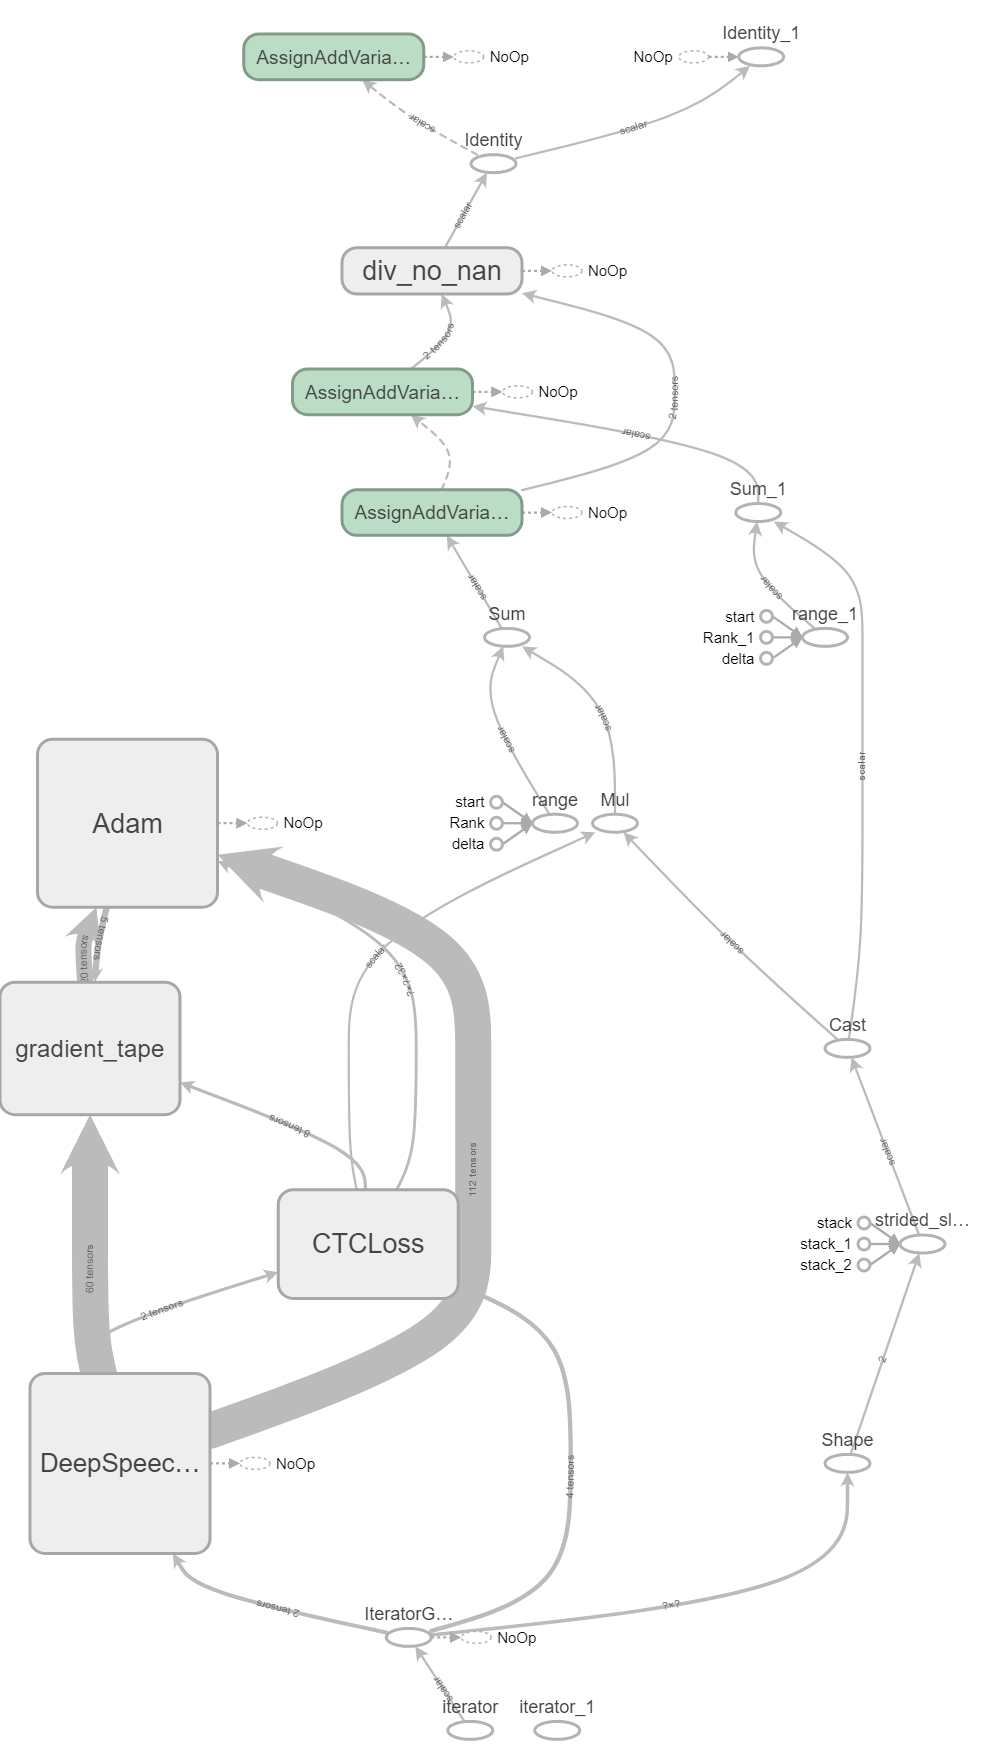
\includegraphics[width=0.7\textwidth]{Figures/model.png}
    \caption[TensorflowModelGraph]{A graph of the general Tensorflow model used in this investigation - deep speech is the name of the neural network outlined above}
    \label{fig:TensorflowModelGraph}
\end{figure}


%----------------------------------------------------------------------------------------
%	BIBLIOGRAPHY
%----------------------------------------------------------------------------------------

\printbibliography

%----------------------------------------------------------------------------------------

\end{document}